\chapter{Who are you?}
\addcontentsline{toc}{chapterdescription}{In answer to the age-old existential question: who am I, and who can I become, you are the forms of thought and meaning\hyp{}making lenses that you use. As in Ubuntu, you are because of other people; optimised for your past, not for your future. Your biggest challenges are adaptive, not technical, meaning you need to change who you are to rise to them. Changing who you are begins with understanding how you deceive yourself, and why this is humanity’s superpower. You can change yourself, primarily through real experiences, not analysis.}
\addcontentsline{toc}{chapterdescription}{\pagebreak}
\label{chapter:who-am-i-base}


\begin{chapterquotation}
The unreflected life is not worth living\\
\raggedleft\textemdash Socrates\index{Socrates}  (at his trial for corrupting Greek youth.) 




\centering
A musician must make music, an artist must paint, a poet must write, if he is to be ultimately at peace with himself.\\
\raggedleft\textemdash Abraham Maslow\index{Maslow, Abraham} 
\end{chapterquotation}


\emph{Who am I?} is the question that follows us throughout our life. 


\begin{longstoryblock}
When I (Graham) was very young, I wasn't even aware of that question. I just lived life as it came, moving through each day, much like an old-fashioned cinema reel moving through the projector. Of course, my life was the typical emotional rollercoaster of any young child. But I wasn't aware of much beyond my immediate impulses. 


I was in balance, the same balance that a pendulum has. I had my ups and downs, but I was constantly moving back to my centre, regardless of whether I was up or down. I certainly wasn't spending long periods of time down caused by buying into my judgements of myself and my environment.


Around the age of six or seven, at primary school, I lost that balance. The pendulum started getting rusted by my judgments about myself. I lost my early childhood capacity to simply let the cinema reel of my life flow without judgement.


More often than not I judged myself as not good enough. Not strong enough, not sporty enough, or too clever. Growing up in South Africa\index{South Africa}, the cultural expectations made it more important to be good at sport rather than classwork. I began shifting my awareness and actions from my impulses in the moment to my needs, which were more stable over time. I began unconsciously constructing myself so that I could better get my needs met.


Striving to get to a point where I could judge myself as good enough, and to get my balance back permanently. For a long time, I thought that balance was a fixed point, that if I got there properly I would always be balanced. 


For a long time I strived to become someone who was good enough, and through that to reach a permanent balance. What made that impossible was that my internal reference frame telling me that who I needed to be, to be good enough, depended on other people. This was something I had absorbed by listening to the norms and expectations of the people and society around me, but these norms were neither self-consistent nor were they consistent with all my facets. 


The result was that I always felt off-balance in a negative way. There was always some part of me that I judged inadequate, that I needed to fix before I would be good enough, and therefore happy.


Over time, I realised that balance is not a fixed destination to reach and then stay at; rather, it's like a pendulum. My objective now is not to reach this stage of resilience where I am never knocked off balance; it is rather to reach a stage of antifragility, where every time I get knocked off balance I am able to get back into balance fast and, more importantly, use the experience to increase my capacity to get back into balance.


I was also growing up within the broader social context of the final decades of apartheid South Africa.\index{South Africa!apartheid}  The older I got, the more aware I grew of how wrong the world I lived in was not only morally wrong, but simply not viable long term. Apartheid could never build a stable society served by a healthy economy. I grew up in a context of fear and anxiety because I knew that apartheid had to end within the next decade or two, and could not see any reason to hope that it would end without extreme pain and turmoil.


And yet who I am today, much of what I am proud of, could only have happened because of how my past has shaped me. One example: the motto of the Eastern Cape school I attended, Selborne, is “Palma Virtuti” (the reward is to the brave), which has occasionally helped me keep going on the path that led to this book. Especially knowing that bravery is not about feeling no fear, it is about doing what needs to be done when filled with fear and doubt. 
\end{longstoryblock}


This background context was like being in a turbulent river, with the current constantly pulling my balance downwards, towards self-doubt, fear, and anxiety.


I described in the first chapter how those experiences are now part of my antifragility. I'm living now in the context of climate change, resource depletion, and all the other signs that the way we are living today is simply not viable for the long term. I look around me, and I see many people who feel anxious about their future. The younger you are, the more anxious you are likely to feel, and the more fatalistic or nihilistic you may be, because you don't see any reason to hope that you will be able to thrive long into old age.


There is hope\index{hope}. There is always hope. 


This and the following chapter offer our suggestions for you to develop your personal capacity for antifragility\index{antifragile}, so that you can harness everything that is stressing you to grow your own personal power. By growing your own power, and your capacity to collaborate with a diverse spectrum of other people, you will be better able to do what is needed to address today’s challenges. And by acting together, we will create our path out of the mess we are in now, to a viable way of living and a better world where we can all thrive.


To grow your personal power\index{power}, the first step is to pull apart the question “who am I?” By doing this you will become better at recognising clearly who you are and who you have been so that you can create the experiences you need in order to grow into who you can become. The “you” that has the personal capacity for antifragility\index{antifragile}  to thrive and take the needed action.






\section{Sense then meaning making}
\label{section:yin-yang-dao}


The most actionable way I've found to look at the question \emph{“Who am I?”} is as the integration of three elements.


\begin{enumerate}
\item Your genes, their epigenetic expressions, and brain structures shaped in early childhood (hardware and firmware) fix your fundamental uniqueness, your natural strengths and weaknesses. 
\item You assembling raw input into complete puzzles that make sense, with the puzzle pieces coming in from all your senses, and including feelings.
\item You then giving meaning to the assembled puzzle through your meaning\hyp{}making stories.\index{meaning-making stories}  
\end{enumerate}


These three are the foundations of the Constructive Developmental Framework\index{Constructive Developmental Framework}  (CDF), described comprehensively by Otto Laske\index{Laske, Otto}  in two volumes\cite{laske-vol1,laske-vol2}. The CDF is the basis in this book for you to get to know who you are, and how you can grow into your potential of who you could become by getting ever more fluid in the thinking you can use, by growing your stories, and by becoming more subtle in how you work with and within the boundaries formed by your fixed nature.


If you know yourself through each of these three lenses\index{lens}, and how they have changed over your lifetime, you will know who you are, who you might become, and most importantly, what to do to become your best future self. Figure~\ref{fig:yin-yang-dao} represents the three elements of stories, thought forms, and genes. 


\begin{SCfigure}[0.9][htb]
%\begin{wrapfigure}{O}{0.45\textwidth}
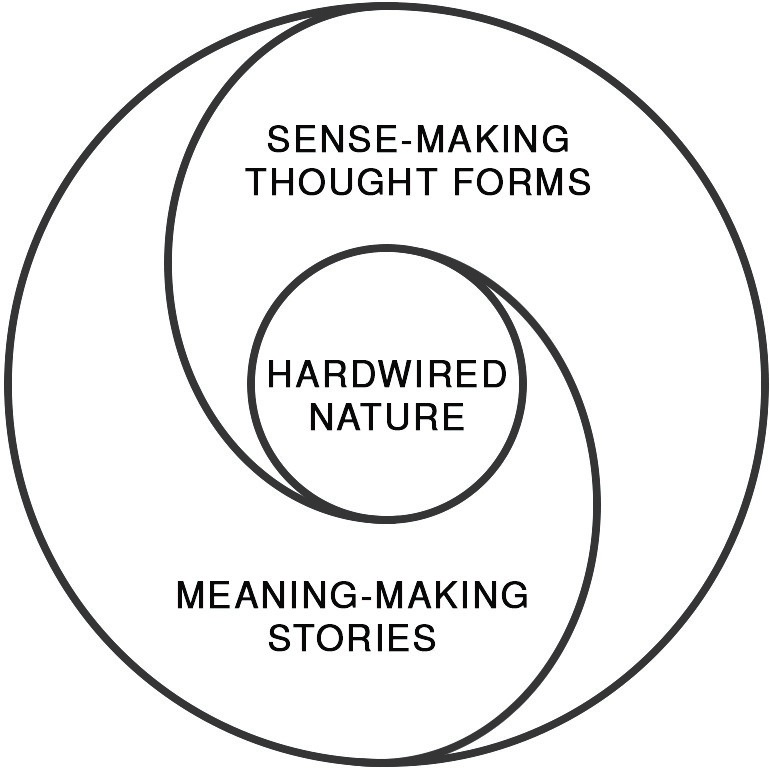
\includegraphics[width=0.42\textwidth]{./Images/yin-yang-dao}
\caption[Three elements shaping our reality and driving behaviour]{The three elements that create our experienced reality and drive our behaviour. Most of these three elements are hidden from us; we are subject to them. The more ability we have to shift them into objects we see clearly, the bigger our adaptive capacity to change ourselves.}
\label{fig:yin-yang-dao}
%\end{wrapfigure}
\end{SCfigure}


I have borrowed Figure~\ref{fig:yin-yang-dao} from Dao/Tao philosophy.\index{Daoism}  It captures, in one simple diagram, how every element of you is interwoven. It makes clear how separating the CDF into three constituent elements is at times a helpful simplification, but it also hides how everything is interwoven. It shows that there are elements you can name and know about and elements that are unknowable and unnameable.


Each of the three elements in the Figure~\ref{fig:yin-yang-dao} plays a distinct role in your experienced reality. They each act in sequence; however, like the way particles interact in quantum mechanics, the sequence happens in very rapid loops that merge into one experienced reality.


First, you receive data into your brain, from your physical senses as well as from your inner ways of knowing. In any instant you can only take in a very small fraction of all the data that is bombarding your senses every second\textemdash for example, your gut telling you that somebody is lying to you.


Then, you use your thoughts to assemble that part of the data that fits together into a representation of actuality, much like putting the pieces of a puzzle together into a final image. Then you use your library of stories to recognise, or project meaning into, the picture on the puzzle you have assembled. This is the reality that you experience.


In Figure~\ref{fig:yin-yang-dao} there will always be aspects of yourself that you are unaware of, and so subject to. The best route to growing bigger is to shift, step by step, what you are unaware of in yourself and subject to, into things that you are aware of and can make an object that you can work with, and then maybe change. 


Norman Wolfe\cite{wolfe-tlo}\index{Wolfe, Norman}  uses the metaphor\index{metaphor}  of a cinema. You can think of yourself and the reality you experience as having four sequential steps that change what actually is, leaving what you experience: (1) the white light, which is everything that is in your potential; (2) the film that filters the light, removing almost everything; (3) the lenses focusing what little is left of the light into an image that you can see on (4) the screen, which itself changes the image.


Depending on your religion or philosophy, the white light represents the universal oneness, the infinite universe, Dao/Tao,\index{Daoism}  God\textemdash all that can be. The reel of film represents the stories that you are. The film that has already passed the lens is now frozen, these are the experiences you have already had. The film that is still coming is not yet fixed. But it is constrained in what's possible, based on your genes and epigenetics, and the large-scale patterns of the time you are living in.


The lens\index{lens}  and screen are formed by everything and everyone around you, enabling you to experience your reality. Unlike in a cinema, these are not neutral, distortion-free flat white surfaces. You have your own unique lens and screen shaping the reality you experience.


One immediate consequence of this analogy is that you can never experience the same reality as anyone else around you. 


You also have three ways of changing your future reality. You can work on changing the image in the film before it's formed; you can change the lens; and you can change the screen. Changing the lens and the screen means taking action to change the environment you are living in, to be with different people, or to go on a mutual journey of change with the people you are with.


To know yourself through each of these three lenses means, firstly, growing your capacity for awareness so that you can be aware in each moment of many more aspects of who you are now and who you once were. Secondly, it also means knowing the frames of reference\index{frames of reference}  you use to evaluate yourself and your actions.
\section{You change yourself by looking at yourself}
\label{section:dressed-you}
One big leap made in quantum physics\index{physics!quantum}  was the realisation that the observer and the observed could not be separated: that the act of observing, independent of any measurement, changed (or even created) what was observed. A photon showed up as if it were a wave or a particle depending on what it was ‘seen’ by.


As soon as you observe yourself by turning your awareness onto one or more aspects of yourself, you immediately change yourself. Who you are now includes who you are in awareness of that part of you that you are observing. Your nature, your capacity for different forms of thought, and your stories about what is and is not acceptable for you to be, shape your self-awareness. So being able to use a well-structured framework makes it much easier to grasp who you are without bias, and to better grow yourself into who you can become.


This is analogous to Picasso\index{Picasso, Pablo}  realising that the very act of looking at something, in order to paint it, shaped what he saw, and later what the person looking at his painting saw. So if he wanted to represent the deeper essence, he needed to break out of the conventional perspective. Just as physicists realised that, to describe nature, they needed to go beyond the biases and limitations of classical physics. 


Keep this in mind, throughout this chapter and the next. You are far more than, and different to, whatever \emph{you} you are currently aware of. You are constantly changing, and every time you focus your awareness on yourself, simply by doing that, you change yourself. Self-identity has a nebulous, uncertain nature, with many parallels to the natural world described by quantum physics.


This means that the full \emph{you} is always different to, and more than, the \emph{you} you can currently be aware of, and there is always more on the edge of your potential to grow bigger. That's the good news. What is challenging for everyone at some point in their life, is the uncertainty of not being able to precisely pin down one single answer, unchanging and valid for all time, to the question \emph{Who am I, and who should I be?}


I'll call this the \emph{naked you} vs. the \emph{dressed you}, borrowing from the concept in physics of dressed vs. naked particles. Every time an electron does its stuff, it's the fully dressed electron. (This is the electron after all the quantum effects coming from its environment have modified its properties. No one ever can see the naked electron.)


How you show up in the world, how others experience you, is always dressed. You experience yourself, dressed by all your stories, the expectations you have of yourself, and the expectations other people have of you. You show up dressed by all your memories, the meaning you make of them, and your hopes and fears about the future.


Growing your capacity for awareness enables you to see more and more clearly everything you are as the fully dressed \emph{you}, and to know that this is the real \emph{you}. The smaller your capacity for awareness, the more likely you are to mistake a small part of your fully dressed \emph{you} for being all you are; or, to seek your naked \emph{you}, which is fundamentally impossible to see.


Your dressed \emph{you} is inherently nebulous, like a cloud changing shape each time you look at it, because each time you look at it you change microscopically your stories, which changes the dressed \emph{“you”}.


This is related to how our memories work. You never actually remember an event, rather you remember the last memory you had of it. Which is why ten different witnesses to a crime give the police ten different, even contradictory, statements. Which is why it is so easy to create completely false memories, as Elizabeth Loftus\cite{loftus-false-memory-ted,loftus-false-memory-wiki}\index{Loftus, Elizabeth}  has shown. Our memories are unreliable, and we can easily acquire a completely false memory, either alone or through the influence of others.


The fact that memories are nebulous, changing each time you remember them, is really good news! It means that you are not destined to stay as you are for the rest of your life. You have changed, you are changing now, and you will change tomorrow.


Because you always have untapped potential to change, to grow bigger, in your own unique way, you always have a reason to hope\index{hope}, and you always have work to do in order to turn that hope into fact. The bigger you are as a person, the bigger your capacity to regenerate yourself after any setback, or to address a new challenge that you have never seen before. 


If you are feeling too small compared to the challenges you see ahead of you, this chapter and the next will show you how to break that judgement down into the small, actionable steps that you can take to become bigger than the challenges you are facing. In the rest of this chapter, you will see a framework that I have found the most useful to understand who I am, and I believe you too will find it powerful for yourself. The next chapter will show you how to use the framework depicted in Figure~\ref{fig:yin-yang-dao} to continue growing into who you can be.


In the next three sections we will work backwards through the sequence. We'll start with your final step in shaping the reality you experience, projecting meaning onto the puzzle your thoughts have just assembled.


\section{You are your stories, thoughts and genes}
Every time you answer the question \emph{Who am I?} you are repeating, adding to and changing your story. The more nuanced and elaborate your story, the bigger you are as a person. 


Over the past few decades research into personality is confirming that, in a very deep sense, your stories are who you are. You have constructed these stories over your life, and they in turn have constructed your personality and the reality that you experience now. You are a dynamic path across time, not a static thing in time. Analogous to quantum mechanics. You construct your stories by distilling the reality you experienced across your life path into scripts defining who you are and what you should do for whom, which then shapes or even creates the reality you experience, which in turn shapes and creates the stories that run you\cite{BBC-life-story,McLean-stories}.


In addition to the stories that you have constructed during your life, and that then construct who you are, the other two elements play an equally important role in who you are: how you think, and your genetic make-up.


How you think, in other words which forms of thought you are more or less fluid in using, determine what you can think about. The kinds of stories that you have access to (out of all the stories you potentially have access to) depend on how fluid you are in each different form of thought. For example, if you are not yet very fluid in using forms of thought around constant flow, movement and change, you will tend to strive towards a fixed self, and then try to stay there. 


The more fluid you are in using constant flow forms of thought, the more you can broaden your stories of who you are to stories describing yourself as a process across time, rather than a self that is a fixed destination, or goal to achieve.


The foundation and boundaries to the potential \emph{you} are given by your genes. You cannot change your genes through force of will\textemdash not yet, at least. Which of these genes are actually active, i.e. expressed, depends to some extent on factors that you can influence, through your diet, your stress levels, sleep and many other factors. How much most of us can change our epigenetics, i.e., change the expression of our genes during our lives, is relatively limited. This means that our stories and our fluidity in using different forms of thought can at best take us to the edges imposed on us by our genes, with some stretch in their epigenetic expression.


\subsection{Ubuntu and the observer}
\label{section:ubuntu}
\begin{quote} I am because we are, \end{quote} or \begin{quote} I am because you are, \end{quote} are the two common English translations of the Ubuntu philosophy. This philosophy has much in common with Picasso's\index{Picasso, Pablo}  art and quantum physics.


Ubuntu recognises that none of us can become human, none of us can become ourselves, without the influence of everyone else around us. Ubuntu\index{Ubuntu}   reflects the full interconnectedness of everyone and everything. The meaning\hyp{}making stories that define who you are today have been shaped by everybody who you have interacted with, and the people they have interacted with, going back many generations into the past. This interconnectedness is at the very heart of what it is to be human. It’s something to embrace and work with.


Who you are now, and how you show up in the world today, shapes who everyone else around you is, and is in turn shaped by who everyone around you is. This means that who you are\textemdash the meaning\hyp{}making stories that shape you\textemdash are not exclusively yours to control. 


You've undoubtedly noticed that with some people it's easy to show up as a bigger, better self, and with others it's hard. Much like the observer in quantum physics\index{physics!quantum}  shapes the specific nature of the photon they observe, your nature is shaped by the people you are interacting with.


Because you are you through other people, the following reasons to hope\index{hope}  and ways to grow yourself emerge.


\begin{enumerate}
\item You can see yourself with compassion because much of who you are could not have been different, and is due to the time, culture, environment, and family you were born into. Your path from embryo to today required you to create your stories of who you are, using the only raw material you had.
\item You can see yourself in the future with compassionate hope because you now have the power to step away from being subject to the stories around you. Instead, you can see your story more and more as an object to influence and shape consciously.
\item You can choose to spend more time with people who help you show up as your bigger, better self; and less time with those who pull you back into being the smaller person that you used to be.
\item You can begin taking yourself and other people less seriously; you can show up in life more playfully, because you know that the potential \emph{you} is much bigger than your current reality. You can improvise and play with alternative stories.
\item You can work more collaboratively and compassionately with other people, because you can see more and more clearly how who they are has been and is being shaped by the people around them, including you. 
\item You can stop blaming yourself and other people for being who they are, and shift your focus to what you can do to step-by-step change the context of your stories, their stories, and how the stories interact with each other.
\item Whilst you cannot become whatever and whoever you want to (because of constraints imposed by your genes, epigenetics, and your past) you can feel hope and optimism that you can become much more than you imagine possible today. 
\end{enumerate}


Picture the difference between a traditional landscape, with its strict perspective, and a landscape by Picasso. Then apply it to yourself: you have far more capacity than you can imagine to step out of the strict perspective of who you are and should be, of what you should do for whom, by channelling the art of Picasso\index{Picasso, Pablo}. He recognised that a painting is there to interact with the observer, who is as vital to creating the reality of the viewing experience now as the artist was when painting. 


To maximise the outcomes it was vital for Picasso to go outside the tramlines of strict perspective. Do the same, and you open up far more power to change yourself and the world you live in for the good.


It was not crucial to your living a good life, up until a few decades ago, to work with yourself more as if you were a Picasso painting than a traditional landscape. In other words, to work with the nebulous changing form or essence of who you are, rather than just your behaviours; and to keep adapting, growing your essence.


It is now essential, because our world is facing global challenges that are so interconnected that there is no way of predicting what might happen in the economy or politics next week, let alone in 10 years. We’re living in a VUCA\index{VUCA}  world of volatility, uncertainty, complexity, and ambiguity, which demands you to be more like a Picasso painting and less like a landscape, so you are best able to recognise and grasp the opportunities to act in the face of these nebulous challenges.
\section[You are optimised for past challenges]{You optimised yourself to overcome your past challenges}
\label{section:optimised-self}


It's not just unhelpful, it is also simply wrong to blame yourself for any aspect of who you are today. 


You have always done the very best you can to optimise who you are to overcome the challenges in the reality you have experienced. The more skilled you become at using the Adaptive Way (described later in this, and in the next chapter), the more clearly you will see the challenges ahead of you, and the more options you will see for who you can become to overcome those challenges.


If you use the cinema analogy, you will realise more clearly that who you are now, and the reality that you now experience, is emerging and shaped by the reality that you have experienced in the past. Never doubt that you have always done the very best you could do, given the situation you were in at the time. Never doubt that you can adapt; that you can continue to learn and grow new ways of acting and reacting. Our lives are non-ergodic paths, like in Section~\ref{section:ergodicity}.


Over the course of your life, perhaps even from before you were born, you began learning how to overcome the challenges that you were experiencing. Everything you experienced in your reality was distilled into the essential lesson about how to thrive, and then either added to your existing stories defining who you are, or you added a new story to your library of stories.


Every time you face a new challenge, you decide whether to engage this challenge by reapplying one or more of the stories that has worked for you in the past, or to let go of everything that has worked for you in the past and figure out how to overcome this challenge from scratch.


It clearly costs you far less time, effort, and energy to overcome today's challenges by reapplying what worked in the past. However, that can only work if today's challenges are close enough to your past challenges for the same solution to work.


All life learns to be ruthlessly efficient with energy. If you run out of physical energy, your physical body dies. If you run out of emotional and psychological energy, you are quite likely to sink into a motionless ball of misery curled up on the sofa bingeing on Netflix and Pringles. So taking the risk to create completely new stories from scratch is a high-risk strategy because it has a high demand on both your physical and psychological energy.


So what should you look for, to decide when it's time to take a blank section of film and write a completely new story from scratch? When the challenge that you are facing is an adaptive challenge, not a technical one.
\section{Adaptive vs. technical challenges}
\label{section:adaptive-technical}


The essence of a technical challenge\index{challenge!technical} is that a technique or technology, and mastery of them, is all you need to fully overcome the challenge. A technical challenge can sometimes be extremely hard to master, but that doesn't make it adaptive.


If it is an adaptive challenge\index{challenge!adaptive}, though, you can only rise to the challenge by changing yourself. You will need to add one or more ways of thinking, you will need to change and grow your stories,\index{stories} and you may need to add more subtlety to how you deal with your hardwired nature. Most likely you will also need to do everything described above for a technical challenge, as most adaptive challenges also have a technical component.


In today's world, much of our pain is caused by trying to address our challenges within our current stories by learning new skills, techniques or buying new technology. But all your VUCA \index{VUCA} challenges can only be addressed if you change yourself. For example, dealing with pandemics like Covid-19 \index{Covid-19} require a fundamental change in who we are being; but almost all effort has gone into medical technology.


We must grow and transform who we are, to build a world we will thrive in. 






One adaptive challenge you have is the first job that you were born with: to become someone. You then become someone by changing who you are from baby to child. And this challenge keeps returning throughout your life. Until you get really good at changing your stories, you will fail to overcome your adaptive challenges, and fall short of your goals, because the barrier to achieving your most challenging goals is in who you are, not external to you. So your focus must be inwards on your meaning making, not outwards on others.


One sure sign that you are facing an adaptive challenge is when nothing you try works, and nothing you can imagine trying looks any better. You feel trapped at the bottom of a 20m well, with no way out. You can express your complaints easily (and often do, at least to yourself), but cannot express clearly what you want and what you can do to get it.


If you are a leader of any sort, most of your challenges will be adaptive challenges. You must become adept at changing yourself and supporting others in them changing themselves. Never attempt to change anyone else directly, though; it will backfire. You cannot write a new story for them; all you can do is support them in creating a context they choose because they believe will facilitate them seeing their own meaning making clearly, and allow it to rewrite itself. No company or manager has the right to demand any specific change in anyone else, they can only point out the business needs and implications of those needs.


If everyone adopts the peer-to-peer practices of the Adaptive Way \index{Adaptive Way} described below, then you have the best available for each of you to adapt yourselves to address these challenges with the least friction, effort, and waste. 


You can categorise your challenge as technical or adaptive using Table~\ref{table:challenge-technical-vs-adaptive}, based on the work of Ronald Heifetz\cite{heifetz-practice}.\index{Heifetz, Ronald}


\begin{table}[htb]
\bgroup 
\def\arraystretch{1.5}% 1 is the default, change whatever you need
\begin{tabular}{p{0.46\textwidth} p{0.46\textwidth}}
\toprule
\textbf {Technical challenges} & \textbf {Adaptive challenges} \\
\midrule
Easy to identify. & Hard to identify, and so easy to deny \\
Easy to solve, best or good practice solutions exist & No existing solution. Can only be solved by changing your stories and thinking, especially your relationships to people, work, and how you see yourself in your roles \\
Experts can give you the solution & You have to do the work yourself \\
Only a few changes within your existing stories and boundaries are enough & Change everywhere, especially to your stories and boundaries \\
It's easy to see and buy into the technical solution & You are unwilling or unable to see the challenge clearly, and that technical solutions are incapable of solving the challenge \\
The solutions are relatively quick to implement & The solutions take time, demanding repeated prototypes and learning from failing until a viable solution is found \\
\bottomrule
\end{tabular}
\egroup
\caption{Technical vs adaptive challenges} \label{table:challenge-technical-vs-adaptive}
\end{table}


To lead yourself and others through an adaptive challenge, Heifetz  identifies five principles. All five are provided by the Adaptive Way practices here and in\cite{boyd-regenerate}.


\begin{enumerate}
\item Look at your stories\index{stories}, assumptions, beliefs, and values. Focus on exploring yourself first, never fixing yourself.
\item Keep the stress levels within a range you and others can contain. Hence the three Evolutesix \index{Evolutesix} dojo rules are critical: care for yourself, care for each other, and care for the whole\footnote{These come from the work of Marilyn Hamilton\index{Hamilton, Marilyn}  on what makes excellent cities different\cite{hamilton-integral-city}. These three are embedded in the city’s culture.}.
\item Identify the themes that most trigger you and keep these smaller than your trigger threshold so that your defence mechanisms, such as denial, blame, or shame, never kick in. Use the patterns in this book.
\item Take personal accountability for adapting yourself.
\item Pay attention to those voices inside you, or actual people around you, who ask challenging questions.        
\end{enumerate}


\section{Self-deception and hope}
\label{self-deception}
Self-deception\index{self-deception}  is a vital superpower coming out of our stories. \emph{“What? I never deceive myself,”} you may think! Take it from me, you do\footnote{This video from Robert Kegan\index{Kegan, Robert}  describes how we practice self-deception well. \url{https://www.youtube.com/watch?v=FFYnVmGu9ZI}}. We are all very good at seeing what isn't there\cite{wiseman-paranormality}. We have to be, because our survival has always depended on the capacity to keep hoping for a better future when times are tough. 


This capacity for self-deception kept Elon Musk investing his last money into both Tesla and SpaceX, splitting it evenly, even though each needed more than he had in total. His hope and illogical decision in the face of the available facts was essential for both Tesla and SpaceX to keep going for a few months longer. By keeping both going, both benefited from unpredictable lucky breaks. 


Paul Ormerod's book\cite{ormerod-why-fail} \emph{Why things fail}\index{Ormerod, Paul}  shows that the dominant reason for business failure is bad luck, i.e., unpredictable negative events, and the same applies to each of us. If you can just stay hopeful enough to keep going, if you can keep the business alive when things are going badly, you may still be around when a random positive event happens. Long-term success and failure depend on ‘lucky’ and ‘unlucky’ events. 


\begin{quotation}
Your capacity for self-deception is the superpower behind your success. Never lose this.
\end{quotation}


But in other contexts, your capacity for self-deception is your ruin, because you either fail to even see fatal risks, or fail to see them clearly. Our risk-lenses, especially in the chaos during great shifts, are poor\textemdash we need better lenses of chaos\index{chaos}. The art of being an effective human is learning how to tell the difference between the contexts, and the opportunities and risks\cite{schrager-brothel} in each context. To see clearly contexts where you are harmfully deceiving yourself about the true nature of actuality\index{chaos}. To see when it's time to apply the philosophy of \emph{winners quit often} rather than \emph{winners never quit}\cite{godin-dip}.


This is especially important in leadership roles\cite{arbinger-leadership}, because other people, perhaps a very large number, will suffer if you cannot tell when self-deception is helpful and when it is harmful. Read more in Section~\ref{section:empiricism}.


Master all the patterns in this book and you have a better chance of recognising whether your self-deception is likely to help or harm you. These patterns, anchored in the best empirical studies, are designed to guard against self-deception in people like me, and perhaps you, who believe in making the world a better place.


Most importantly you will be able to continue feeling hopeful when facing huge odds, or at least continue to act as if you felt hopeful, even if you feel anxiety or despair. The more you can do this, the more power you have to overcome the adaptive challenges that you are facing, and will continue to face. 


\section[Experience changes you, not analysis]{Experiences changes your stories, not analysis}
Your history, and what you've experienced in your past, is almost irrelevant in becoming who you have the potential to become. This may seem surprising to you, given how much focus there is on analysing past experiences. However, research in psychology is showing with steadily growing clarity how widely different the histories are for people dealing with the same meaning\hyp{}making stories; and that rewriting those stories depends more on the growth experiences you construct now, and far less on having a deep understanding of your past. 


For many, understanding their past is often irrelevant; and may even be harmful, because your memories have become too distorted from your actual past.


This means that there is nothing to stop you from starting work today on creating the experiences that you need to adapt yourself in order to rise to your adaptive challenges\index{challenge!adaptive}. Dive into Chapter~\ref{chapter:who-am-i-meaning} to begin doing this work on yourself now, if you want to.


Most of us, though, find it helpful to understand the patterns in our past that have got us to who we are today. I have certainly found it helps me act more compassionately towards myself, my family, and the people who used to bully me at school. So I do invite you to use this chapter and the next to develop understanding. But don't expect that understanding alone will have much impact on you becoming who you can become.






\section{So who ought you grow into?}
Most of the old approaches to developing oneself recognised that there are many paths to self-mastery, wisdom, and enlightenment. Think of a monastery (maybe you enjoy Ellis Peters’ Cadfael books); the monk’s spiritual development is throughout their daily work. Whether they are reading the Bible, washing carrots, or like Cadfael solving the mystery of a dead body embedded in the ice, it's all part of developing themselves and being of service.


What they realised is that we all live on unique paths. Our lives are inherently non\hyp{}ergodic, like in Section~\ref{section:ergodicity}. All your good fortune and bad fortune in your history is part of the unchangeable path you have been on up to now. All you can influence is your future, starting with where you are now on your unique life path. You cannot change your past, give up all attempts to change your past. (And much of what we all do is ineffective because at core it’s saying, for example, \emph{“If he would only apologise, then my past would be different and I’d feel fine”}. 


No-one else has been on exactly your life path up to now, nor can you access any of the other possible life paths you might have had if fortune had favoured you differently. Life is inherently inherently non\hyp{}ergodic, which is why it is, to a greater or lesser extent, wrong to imagine that you have had the same chances to make something of your life as someone else has. Your unique life\hyp{}path sequence of good and bad fortune has uniquely privileged or disadvantaged you compared to someone else. Which is also why it cannot help to compare where you are now to someone else; you never can know what different sequence of good or bad fortune has made all the difference. 


A powerful component of your life path, that you can harness to grow, and create a better future life path for yourself, is your work, and the conflict you experience at work. It is as necessary a part of you getting to know yourself and developing yourself as reading this book, actively reflecting on your experiences, or any other developmental practice\cite{laske-vol1, sen-development}.


This is very clearly evidenced in all the research into what has made highly successful companies remain so over decades. In them, work contributes so powerfully to each individual developing themselves and their natural talents that the best people want to work there. These are the companies that recognise that fighting the war for talent is a sure way of losing it. It's not a war, it's a garden. Provide all the right conditions, and you will grow top talent out of everything that arrives, and will attract the most ambitious people who are driven by developing themselves. Growing talent collaboratively gives you far better long term performance than hiring talent in a competitive battle.


Knowing whether you are truly developing yourself, or meeting the expectations of other people to be what they want you to be, is a challenge without a simple answer. The best you can do is follow Polonius\index{Polonius}  (councillor to the Danish King) words when he counsels his son Laertes in Hamlet\cite{shakespeare-own-self}: \begin{quote}This above all, to thine own self be true, and it must follow as the night the day, thou canst not then be false to any man\end{quote} 


Despite Shakespeare poking fun at Polonius’, this advice has stood the test of time. But what does it mean to be true to thine self? And how can one know oneself? In a sense, because knowledge is always under construction, who you are is always under construction in every moment, and so you will only know how you have been true to yourself looking back. The best you can do in the moment is lean away from your current context and look far into your past and future.


\begin{longstoryblock}
How I (Graham) apply this quote is the same as the way I learned how to ride a motorbike or climb the vertical faces of Table Mountain\index{South Africa!Table Mountain}. On a motorbike, when you go through a corner, the faster you’re going, the less you look at the corner, rather you look as far around the corner as possible to where you are heading. Amazingly, by not paying attention to where the motorbike is now and what's happening now, but rather paying attention to where you want the motorbike to be as far into the distance as you can see, you magically avoid all the hazards in the moment.


When I was climbing, whenever the climb got tense, the mantra I used to relax and find a way through was \begin{quote} when in doubt, lean out. \end{quote} By leaning away from the rock face and into danger, at the point where I was starting to tense up and pull myself into the rock face, I was able to get a better overview of everything else the rockface offered me.
\end{longstoryblock}


Look as far into your future as you can. Lean out of your immediate panic and look at what else your current context offers you. Do this and you're more likely to recognise your unique path growth, not somebody else's.


And sometimes, you will need to step across a misty void, with nothing secure under you. You will need to leave behind everything that was secure, and what will be secure is not yet in sight. This is a kind of mini-death, leaving your old self behind before you have any idea of who you need to become. 


You have two choices. Keep going, or retreat. Choose with your best long-term wisdom. 




\section{The Adaptive Way: How to grow bigger than your challenges}
I (Graham) developed the Adaptive Way\index{Adaptive Way}  with colleagues in Evolutesix \index{Evolutesix} over the past ten years by integrating many different evidence-based approaches, and transforming them into one peer-to-peer way of interaction. The primary objective was a way based on dialogue that can be used at work, regardless of anyone’s beliefs or religion. 


Whether you are interacting with your colleagues at work, with your friends and family, or with the different aspects of yourself, these are powerful patterns to harness tension and conflict in service of your growth. 


It’s called “way”, for the same reason Aikido and many others have “way” in their name: this is primarily a way of being and living, not a technique to master. Just as in many of the martial arts, there are patterns to become fluid in. Your end goal is to become so fluid in them that you achieve unconscious mastery, where you are no longer aware of your mastery, and you use just the right variation of pattern in the moment.


The intent and spirit of the Adaptive Way has much in common with Aikido. Both are centred on conflict, and both see conflict as a war \emph{with} oneself that you can use in order to grow in power \emph{to}, not as war \emph{against} another to exert power \emph{over}.


In today’s world, our common approaches to conflict\index{conflict}  are always a net loss. They assume that the only relevant capitals are financial and territorial. That is certainly false today. So even if you win the narrow conflict in the financial or territorial sense\textemdash say you get a higher rate of return from some business deal at the expense of other stakeholders\textemdash the cost across all capitals leaves you and / or your children worse off long term. Such lose-lose-lose ways of war are long past their sell-by date. 


The Adaptive Way is part of the art of war that’s needed to defend and grow the capitals of life, both human and natural. And this begins first and foremost with you: master them to grow yourself into the biggest, most developed version of yourself according to your life path and nature. 


Again, you need multiple lenses, because the Adaptive Way transcends and includes all the either / or paradigms of common practices. Just as much as the Adaptive Way is a soft, meditative, mindful way of self-development, it is also the way of the new warriors that we need, in order to have regenerative businesses and a regenerative economy. The next three chapters introduce the Adaptive Way, and the forthcoming books, and Evolutesix application programmes, go into detail. 


\begin{quotation}
Please stay safe whenever you work on yourself and interact with others. Firstly, make sure that the rules of a safe Dojo are well applied, because everyone is willing and able to apply them, and because you have a more adept practitioner to support you in staying safe. Secondly, keep in mind that (like a vulnerable scorpion after shedding one exoskeleton, but before hardening the next) you are at risk of exploitation by any malevolent narcissists, psychopaths, etc. in your orbit. Keep a careful eye open for signs of these. For signs of people who will harness your vulnerabilities to serve themselves.
\end{quotation}